\section{Data Acquisition (DAQ)} 
\label{sec:daq}

%%%%%%%%%%%%%%%%%%%%%%%%%%%%%%%%%%%%%%%%%%%%%%
\subsection{Scope and requirements}

%This section outlines the data acquisition (DAQ) for ProtoDUNE-SP.
The data acquisition (DAQ) system is shown in Figure~\ref{fig:daq-overview} along with its
interfaces to the cold electronics, beam instrumentation, and online
computing systems.
\fixme{Figure~\ref{fig:daq-overview} requires significant zooming to read.  Need a simpler 
diagram initially to show the major pieces, and only the DAQ pieces. Also some descriptive text; relate the physical components to data rates and such.}
\fixme{timing, trigger, throttle systems, FPGA-based master, etc.}

\begin{cdrfigure}[DAQ Overview]{daq-overview}{Detailed overview of the
DAQ system, its interconnections, data flow, timing and control signals,
and the interfaces to the electronics and online computing systems}
        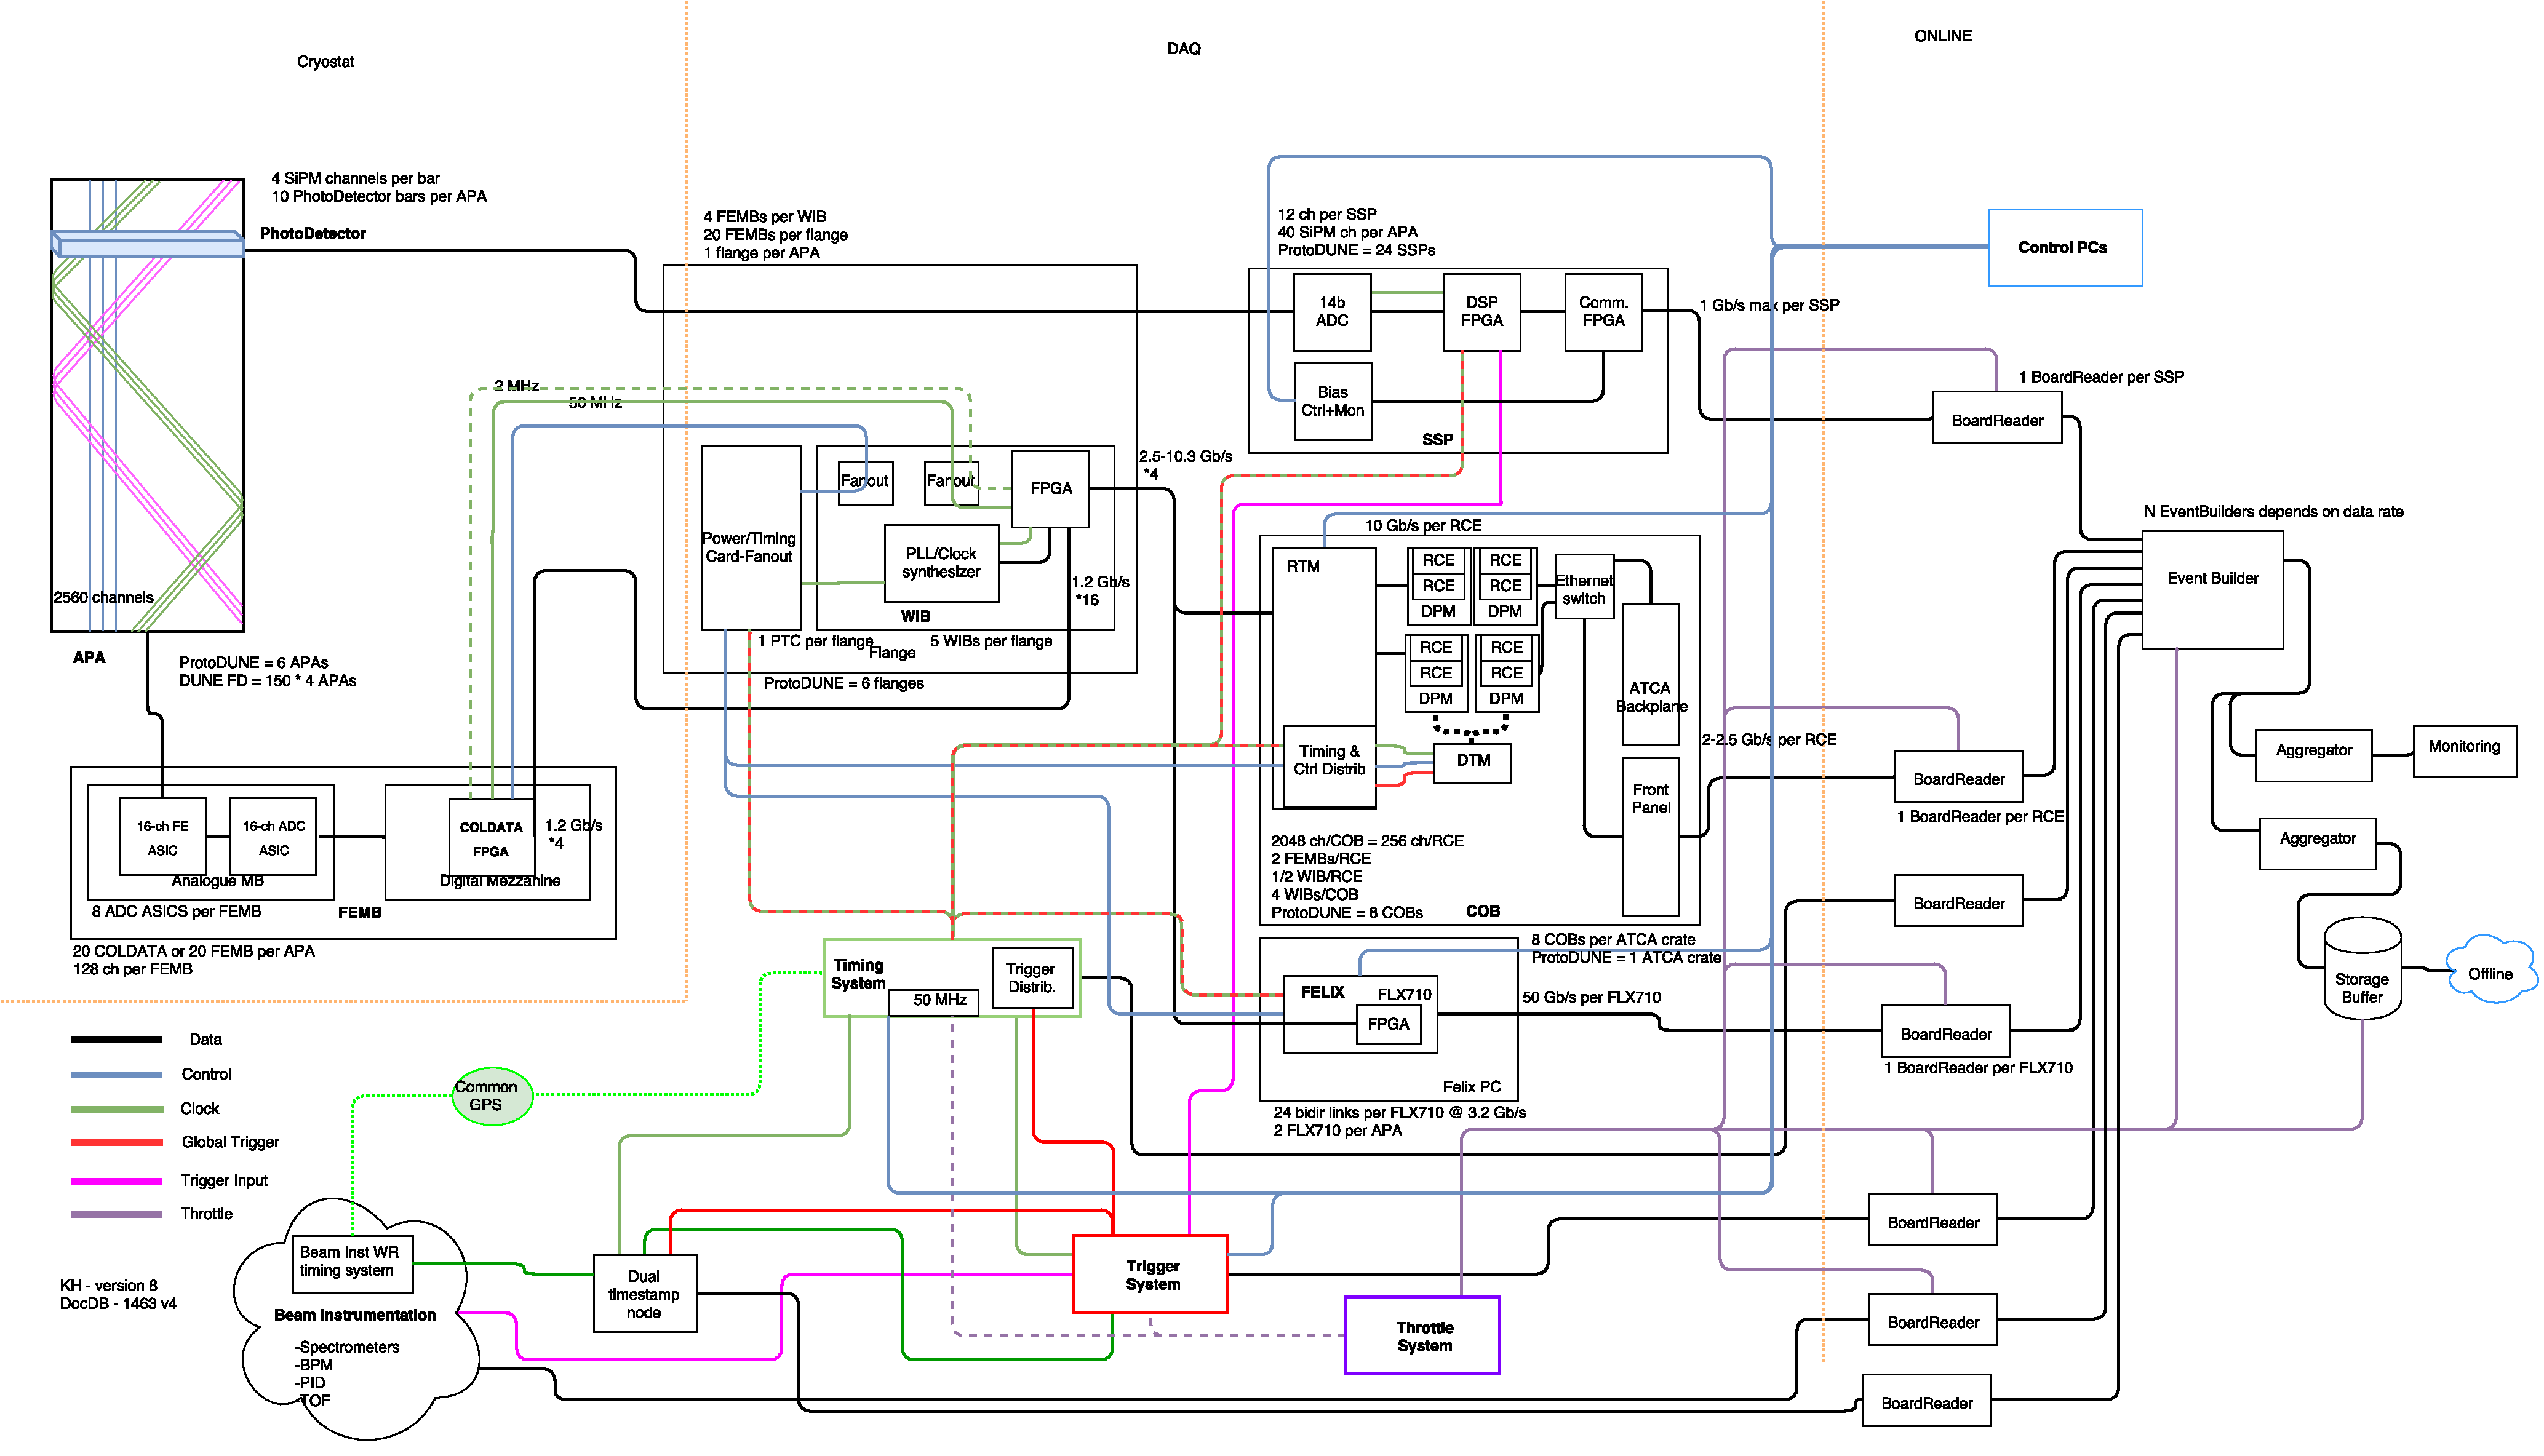
\includegraphics[angle=90,width=0.70\textwidth]{daq-overview-dia.pdf}
\end{cdrfigure}

%The requirements for the DAQ system are definedby the physics requirements of  ProtoDUNE-SP, with constraints from thefront-end electronics and assumed bandwidth and storage requirementsfrom the online and offline computing systems.  The baseline triggerrate during the SPS spill is taken to be 25 Hz.  Cosmic data will alsobe acquired at an appropriate rate such that bandwidth and processing priority are given to beam data.
 
The physics requirements of  ProtoDUNE-SP are the primary drivers of the
DAQ system requirements.
The front-end electronics and assumed bandwidth and storage requirements
from the online and offline computing systems impose additional constraints.  

The run plan (see Section~\ref{sec:runplan}) calls for about 25\,M analyzable beam events
to be collected in the first run of \pdsp. Data sets may be enhanced  in desirable particle types and energies
with dedicated triggers (such as PID)  from the beam instrumentation. The latter is described in Section~\ref{sec:beaminstruments}.

Parameters of the data collection plan are listed in Table~\ref{tab:goldi}. The lossless 
compression factor cited
in the table is based on the assumption that the signal-to-noise level 
is similar to or better than that achieved by MicroBooNE. \fixme{needs citation}


\begin{cdrtable}[Parameters defining data rate and volume in the ``most likely'' scenario]{ll}{goldi}{Parameters defining data rate and volume in the ``most likely'' scenario v5\,\cite{data_spreadsheet}. The buffer depth includes both
  the in-spill and out-of-spill data.}
Parameter & Value \\ \toprowrule
    Trigger rate & \SI{25}{\Hz} \\  \colhline
    Spill duration & \SI{4.8}{\second} \\ \colhline
    SPS Cycle & \SI{22.5}{\second} \\ \colhline
    Readout time window & \SI{5}{\milli\second} \\ \colhline
    \# of APAs to be read out & 6 \\ \colhline
    \hline
    Single readout size (per trigger) & \SI{230.4}{\mega\byte} \\ \colhline
    Lossless compression factor & 4 \\ \colhline
    Instantaneous data rate (in-spill) & \SI{1440}{\mega\byte\per\second} \\ \colhline
    Average data rate & \SI{576}{\mega\byte\per\second} \\ \colhline
    \hline
    3-Day buffer depth & \SI{300}{\tera\byte} \\

\end{cdrtable}
%end insertion from computing-data-handling file

\fixme{Data rates}

 The baseline trigger
rate during the SPS spill is taken to be 25 Hz.  Cosmic data will also
be acquired at an appropriate rate such that bandwidth and processing priority are given 
to beam data.\fixme{this comes out of nowhere}

The data rate from the electronics is dominated by the
TPC data.  However, the photon detection system (PDS) can produce a signifcant
amount of calibration data (where full waveforms are extracted), during
commissioning and special runs (up to 24\,Gb/s maximum).

The TPC data is sent via the Warm Interface Boards  (WIB) on the cryostat flanges
for the six APAs, un-triggered at a total rate of 480\,Gb/s.  
The PDS data is estimated to send data
at a total rate of 1.2\,Gb/s from the 24 SSPs (detailed further in Section~\ref{subsec:pds-readout}).
The maximum bandwidth from the ProtoDUNE-SP online system to CERN IT (and
hence, the offline world), is 20\,Gb/s at a maximum.
Therefore, the DAQ system must reduce the data by a significant fraction
before it is sent offline.  This is achieved by a combination of
data compression and triggering.

%%%%%%%%%%%%%%%%%%%%%%%%%%%%%%%%%%%%%%%%%%%%%% 
\subsection{Timing, trigger and beam interface}
\label{sec:daq_time}

The timing and trigger are two distinct subsystems.  The timing
system provides the distribution for the trigger signals over the same
fabric as the clock and calibration signals.  %Each of the systems willbe described separately, along with a brief section on the interface to the beam instrumentation.

%%%%%%%%%%%%%%%%%% 
\subsubsection{Timing}


The timing system is required to provide a stable and phase-aligned
master clock to all DAQ components; synchronize external signals into the
ProtoDUNE-SP clock domain and time-stamp them; distribute synchronization,
trigger and calibration commands to the DAQ system; and conduct continuous
checks of its own function. In addition, the timing system acts as a
data source, providing a record of triggers received, distributed, or
throttled. The system is designed to meet the full eventual requirements
of the DUNE experiment, but needs only a subset of that functionality
for ProtoDUNE-SP. For instance, absolute time-stamping with respect to an
external GPS reference is not required.

An FPGA-based master unit 
\fixme{is this part of the DAQ?}
receives a high-quality clock signal 
(from a quartz crystal oscillator or external source) 
and external signals from the
trigger system and SPS accelerator. It interfaces to the ProtoDUNE-SP control
and DAQ via a gigabit Ethernet interface. The master unit multiplexes
synchronization and trigger commands, along with arbitrary command
sequences requested by software, into a single encoded data stream,
which is broadcast to all timing endpoints, and decoded into separate clock
and data signals. A uniform phase-aligned cycle counter, updating at the
ProtoDUNE-SP system frequency of 50\,MHz, is maintained at all endpoints,
allowing commands to take effect simultaneously at all endpoints
regardless of cable lengths or other phase delays.

The timing signal is broadcast via multi-mode optical fiber (for
medium-distance connection to the WIB crates on the detector) and LVDS
signals are sent over twisted-pair cable (for short-distance connection to RCEs,
SSPs and FELIX modules). Optical signals are fanned out and recombined
using commercial 32:1 passive splitters, and active optical--LVDS
converter boards further split the signals for local distribution to
endpoints. 

Endpoints decode the timing signal into separate clock and data
signals using a commercial clock-data recovery ASIC ~\cite{siliconlabs:Si5344}, which in turn
feeds a low-bandwidth PLL \fixme{define} in order to remove any remaining jitter in
the clock and provide phase adjustment. The data stream employs 8b/10b
encoding, ensuring sufficient transitions in the timing signal for clock
recovery and correct operation of optical links, and uses scrambling
of idle patterns to minimize electromagnetic interference (EMI).
 A common firmware block is used to
decode the timing protocol, which is incorporated into the overall
firmware design for the receiving FPGA in each DAQ component. This
block provides a cycle counter, several independent trigger, calibration and 
synchronization signals, and a general-purpose packet data output to each endpoint.
The cycle counter is used to generate low-frequency timing signals for
further propagation, e.g., the 2-MHz sampling signal for the cold ADCs.

%%%%%%%%%%%%%%%%%% 
\subsubsection{Trigger}

The baseline trigger solution for ProtoDUNE-SP is the Central Trigger Board
(CTB). The CTB is designed to receive triggers from various subsystems
(Photon Detection System, Beam Instrumentation, SPS spill signal, veto
signals, etc.).  Up to 100 input channels are provided.  It combines
these into a global trigger based on a configurable input mask (or
more sophisticated algorithm, if desired).  It provides functionality
to globally time-stamp triggers, keep event counts, and provide artDAQ-compatible 
\fixme{reference} header information with trigger type and error conditions.
Internally generated triggers and calibration pulses allow for testing
the board itself and the end-points receiving the trigger signals.

The CTB is based on the MicroZed development board~\cite{avnet:microzed}, which comprises a
Xilinx Zynq-7000 System-on-Chip (SoC), 1-GB DDR3 RAM, Gigabit Ethernet,
and 115 I/O ports.  The Programmable Logic of the Zynq-7000 is used to
perform fast triggering operations, whilst the Processing System is used
to interface to the readout and controls systems.

Configuration and operation is performed using an XML file which is sent
to the CTB.  This allows for fast reconfiguration of the CTB without
the need for new firmwares.  The file is used to both configure the board
and send start/stop/reset, etc., commands from the run control.
The trigger output format consists of a trigger type (physics/calibration/random),
a time-stamp, the trigger word, counter information and the values 
of the inputs causing the triggers.  
The trigger system uses the timing system clock and global triggers are
distributed via the timing system.  


%%%%%%%%%%%%%%%%%% 
\subsubsection{Beam Interface}

The beam instrumentation is described in Section~\ref{sec:beaminstruments}.
The beam instrumentation DAQ and the DAQ for ProtoDUNE-SP
have separate timing systems.  A common GPS clock is used to keep both
systems synchronized relative to each other.  A common endpoint receives time stamps 
from both WhiteRabbit (for the beam instrumentation) and the ProtoDUNE-SP timing system
are used to create a matching table from the two systems.  
\fixme{what does the `both' refer to?}
Data from the beam
instrumentation is acquired continuously via a separate DAQ path. \fixme{separate from the actual data?}  Triggered
data for ProtoDUNE-SP have both the TPC, PDS, and beam instrumentation data and 
the timestamps and trigger information of both. \fixme{here `both' seems to refer to 3 things}

%%%%%%%%%%%%%%%%%%%%%%%%%%%%%%%%%%%%%%%%%%%%%% 
\subsection{TPC data readout}

The readout of the TPC wires, prior to being received by PCs in
the back-end DAQ, consists of  CE on the APAs
inside the cryostat and electronics outside
the cryostat, both directly on the cryostat flange and in a rack (the
warm electronics).  This section
addresses the warm part of the TPC
readout and describes how it receives data from the CE (the Front-End
Boards), manipulates the data, and delivers it to the back-end DAQ.

From an electronics point-of-view, the flange (one per APA) consists of a
5-slot ``crate,'' where the connectors on the warm side of the feedthrough 
form the ``back-plane'' into which the boards plug when inserted
into the crate assembly. 
\fixme{crate vs crate assembly?}
  These connectors and the boards that plug
into them (warm interface boards, WIBs) serve to send the power,
timing, and configuration down to the FEBs \fixme{define} and receive the high-speed
signals from the FEBs. From a data standpoint, each WIB receives the
data from four FEBs over sixteen 1.25-Gbps data lines, and multiplexes
this data to four 5-Gbps (or two 10 Gbps) lines that are sent over
optical fiber to the DAQ.

Two systems are used to receive data from the WIBs.  The baseline
solution is based on Reconfigurable Computing Elements (RCE) and 
read out data from five APAs.  An alternative exploratory prototype based on
the Front-End-Link-EXchange (FELIX) system is used to readout the sixth APA.

%%%%%%%%%%%%%%%%%%%%%%%%%%%%%%%%%%%%%%%%%%%%%% 
\subsection{RCE-based readout}
The data from the WIB are received by processing units called RCEs (Reconfigurable Cluster Element), 
\cite{slac:rce}
which are housed in industry-standard
ATCA shelves on COB (cluster-on-board) motherboards that are designed
at SLAC for a wide range of applications.   The RCE is a SoC 
from the
Xilinx Zynq family and contains a full Linux processor system on the chip
accompanied by 1\,GByte of DRAM.   The primary processing functions of the
RCEs are compression (and/or zero-suppression) and buffering
of the raw data and then sending data to the back-end upon the receipt of
an external trigger.  Each COB carries eight RCEs, all connected to each
other via an on-board 10-Gbps Ethernet switch, which also sends data out
of the COB to the back-end DAQ PCs.

The interface with the WIB is provided via the ATCA compliant rear-board, the RTM (Rear Transition Module).  
This application-specific board uses a set of QSFP transceivers to receive
the data from the WIB and an SFP+ (small form-factor pluggable)
 optical interface for communication
with the timing and trigger distribution system.

As the multiplexed data from the WIB comes into the RCE FPGA fabric,
it is de-multiplexed and buffered into per-channel, fixed-time-length 
chunks (for instance 512- or 1024-ticks).  These chunks are
compressed and written to the DRAM where the RCE processor waits
for a trigger (also handled by the FPGA) to arrive.  Upon a trigger, the
processor sends data for a fixed window in time, including pre- and post-trigger time chunks
for all channels, to the back-end PCs.  

For ProtoDUNE-SP, 256 wires worth of data (2 FEBs) are sent to each RCE.
Given that there are 120 FEBs in ProtoDUNE-SP, 60 RCEs are needed to
readout the full detector.  These fit into eight COBs which in turn
reside in a single 14-slot ATCA shelf.

%%%%%%%%%%%%%%%%%%%%%%%%%%%%%%%%%%%%%%%%%%%%%% 
\subsection{FELIX-based readout}
The FELIX is a PCIe card receiving data on point-to-point links from
the detector electronics and routing those through a switched network
to computers.  The aim is to reduce to a minimum any specific hardware
developments and to fully rely on commercial networks and servers to
perform the DAQ tasks.  For ProtoDUNE-SP, data from five WIBs (20 FEBs) is read out over ten 9.6-Gbps links into two FELIX cards.  Grouping
time slices around a trigger signal, as well as data compression, will be
dealt with in software. Similar to the RCE-based readout, the FELIX 
generates artDAQ fragments to be sent to the event builder.


%%%%%%%%%%%%%%%%%%%%%%%%%%%%%%%%%%%%%%%%%%%%%% 
\subsection{PDS and beam instrumentation data readout}
\label{subsec:pds-readout}

%The PDS data rates are described here.  The PDS electronics and DAQ are described in section \ref{sec:pds-elec-daq}.  
A combination of externally triggered events
and self-triggered events make up the PDS data.  The external triggers
come from the beam instrumentation via the trigger system at 25\,Hz.
This amounts to 118\,Mb/s.  The self-triggered data
are induced by cosmic rays.  A cosmic rate of 10\,kHz is assumed,
totalling 1106 Mb/s.
The combined rate comes to $\approx$1.2\,Gb/s.  An alternative scheme with
just self-triggered header-only data with a resultant rate of $\approx$1.1\,Gb/s is considered for implementation if
the former proves difficult.


%%%%%%%%%%%%%%%%%%%%%%%%%%%%%%%%%%%%%%%%%%%%%% 
\subsection{Event-building software }

Developed within the Fermilab Scientific Computing Division and
already used for the 35-t prototype, \textit{artdaq} provides data
transfer, event building, and event analysis functionality. This
latter feature includes built-in support for the art event analysis
framework,
also developed at Fermilab,~\cite{fnal:art}, allowing experiments to run art modules for real-time
filtering, compression, disk-writing and online monitoring. As art is also used for offline analysis, a major
advantage of artdaq is that it allows developers to easily switch
between developing online and offline software.

Artdaq provides three types of processes, each of which
fulfills a specific role. In the order of upstream-to-downstream, these
are boardreader processes, eventbuilder processes, and aggregator
processes. A given boardreader process is intended to be associated   %%%%%%%%%%%% Anne
with a particular geographical region of the detector, and provides
hooks (in the form of C++ base classes) for an experiment's developers
to embed experiment-specific code (called ``fragment generators'')
designed both to upload configuration values to hardware and to read
out the hardware. For ProtoDUNE-SP, the full DAQ will consist of 87+ 
boardreaders, in charge of the 60 RCEs, 24 SSPs, the timing system, 
the Penn Trigger Board, and at least one for the beam instrumentation.
%For testing purposes whenno hardware is available, fragment generators are available whichdon't actually interface to true hardware, but instead perform usefulfunctions such as read in existing output files, extract theirfragments and send them downstream (serving as a "playback" mechanism,essentially) as well as model pathological behavior such as sudden,precipitous increases in data rate or unexpected dropoffs in upstreamdata flow.  (Shorten per Eric J)
For testing purposes, fragment generators can perform useful
functions such as providing a ``playback" mechanism,'' and modeling sudden or unexpected data flow events.

Downstream of the boardreader processes are the eventbuilder
processes. An eventbuilder receives data from every boardreader (a
chunk of data from one boardreader corresponding to an event is
referred to as a "fragment"), and assembles the fragments for a given
event into a raw, complete data event. Optionally, filtering via art
modules can be performed at this stage.

The most downstream process type is the aggregator. Traditionally in
artdaq-based DAQ systems, there are two aggregators, one in charge of
writing data to disk and reporting aggregate statistics (MB/sec,
e.g.), and one in which experiments can run art analysis modules for
real-time online monitoring. 
%
%For ProtoDUNE-SP this model will change asartdaq becomes more flexible; current versions of artdaq supportmultiple diskwriting aggregators which may increase throughputcapability as well as support for multiple monitoring processes whichare decoupled from artdaq. It is possible for much of the functionalityof aggregators to be replicated in eventbuilders; while this reducesthe number of interprocess connections in the DAQ software, adisadvantage of an eventbuilder-only system is that the number ofprocesses assembling raw events is the same as the number of processeswriting to disk.
%
For ProtoDUNE-SP this model will change as
artdaq becomes more flexible and throughput
capability increases. The functionality
of aggregators may be replicated in eventbuilders. While this solution  reduces
the number of interprocess connections in the DAQ software, the number of
processes assembling raw events is the same as the number of processes
writing to disk.


%For the 35ton prototype, artdaq processes were controlled by a program calledDAQInterface. DAQInterface can be thought of as an intermediarybetween Run Control and the individual artdaq processes; it's incharge of launching the artdaq processes and sending themconfiguration code on initialization, and repeatedly querying theprocesses to see whether or not they return an "Error" state; if thisis the case DAQInterface will automatically stop datataking and shutdown the processes in an orderly fashion, so that unexpected behaviorfrom upstream (e.g., hardware suddenly sending an unmanageably highrate of data) will not result in improperly closed output files,zombie processes, etc. For ProtoDUNE-SP, the plan is to shift some of the functionality of DAQInterface (such as querying artdaq process status) over to JCOP (Joint Controls Project); where appropriate/possible, DAQInterface code will be reused so as to minimize unnecessary duplication of effort. 
 
For the 35-t prototype, artdaq processes were controlled by a program called
DAQInterface. DAQInterface takes 
charge of launching the artdaq processes, checking for error states, and
shutting down
 processes in an orderly fashion as needed, to avoid improperly closed output files,
zombie processes, etc. For ProtoDUNE-SP, some of the functionality of DAQInterface (e.g., querying  status) will shift to JCOP (Joint Controls Project);
DAQInterface code will be reused as appropriate/possible, to minimize duplication of effort. 



%%%%%%%%%%%%%%%%%%%%%%%%%%%%%%%%%%%%%%%%%%%%%% 
\subsection{Control, configuration and operational monitoring}

The artDAQ software used for all applications dealing with the movement,
processing and storage of data will be interfaced with software of the
Joint Controls Project (JCOP) for the purpose of control, configuration
and operational monitoring.  JCOP provides a toolkit to implement run
control (finite state machine (FSM), distribution of commands, error
propagation and handling) as well as graphics tools that allow for the
implementation of user interfaces and monitoring dashboards.  In order to
minimize the software development needs the same FSM as defined by artDAQ
will be implemented and commands will be sent to the applications using
the already supported XML-RPC protocol.  Monitoring data will be pushed
into the JCOP framework by implementing the appropriate artDAQ monitoring
plugin.  Log and error messages will be most probably collected and
processed using an implementation of the ELK (elastic search, logstash,
kibana \cite{elastic:kibana}) stack. 
 The internal configuration of DAQ applications will be
carried out using the mechanisms provided by artDAQ. The overall system
will be modeled and configured using the JCOP paradigm (data points).


%%%%%%%%%%%%%%% Tom's stuff
\subsection{Interface of the DAQ to the online storage}
\label{sec:DAQ_online_interface}

%Table\,\ref{tab:goldi} indicates a nominal trigger rate of 25\,Hz for the mid-range scenario. It may be necessary to provide the capability to run at  an instantaneous trigger rate of up to 100\,Hz in order to allow for commissioning and schedule delays. For that reason, scalability of the DAQ, the online buffer and the prompt processing system \ref{sec:prompt_processing} is an important design requirement. Data are assumed to be collected based on prompt trigger signals generated by the beamline instrumentation in order to purify samples of desired particles.
Table~\ref{tab:goldi} indicates a nominal trigger rate of 25\,Hz for
the mid-range scenario. 
 Data are assumed to be
collected based on prompt trigger signals generated by the beamline
instrumentation in order to purify samples of desired particles.

%Current estimates put the PDS data at approximately 10\% of the TPC data rate.  Beam instrumentation data is expected to be lower still. As such, the readout of the photon detector channels and the beam instrumentation is assumed to be a relatively minor addition to the total data rate and are not anticipated to drive the design of the data handling and processing system, although adequate resources must be provisioned in order to acquire and store the data from these systems. 
Current estimates put the PDS data at approximately 10\% 
of the TPC data rate.  Beam instrumentation data is expected to be lower still.
Although adding to the
total data rate only slightly, adequate resources must
be provisioned in order to acquire and store the data from these
systems.  

The network speed of all computers in the DAQ
chain is anticipated to be 20\,Gbits/sec. 
 Computers running near-line
processing of subsets of the data, which are generally CPU-bound, may
be connected with 1\,GBit/sec links.  The software framework for
interfacing with the electronics, building events, writing data files,
and providing an interface to online monitoring of data as it is
acquired is {\it artdaq}~\cite{artdaq}.

%Assuming that each RCE reads out 256 channels of the TPC, 60 RCE's will need to be active.  For the PDS, 24 SSPs will be used.  A number of computers (minimum 2) running BoardReader processes will read out the RCEs.  These computers should be provisioned with 1 core per process, along with a 10\,Gbit/sec network connection.  The BoardReader processes will transmit data to a set of computers running EventBuilder processes. A number of Event Builder computers (minimum 4), with 10-20 cores and a pair of 10\,Gbit/sec NIC will provide the CPU and networking needed to build events, collect basic metadata, and send the data to storage and online monitoring.  The Event Builders assemble data fragments sent by the BoardReaders into self-consistent events consisting of readout data from each contributing RCE, SSP, and beam instrumentation information for the same time period.  They will also perform basic data integrity checks, ensuring that all data that are expected for an event have arrived and have not been corrupted, before writing records out.

Given that each RCE reads out 256 channels of the TPC, 60 RCEs
will need to be active.  For the PDS, 24 SSPs will be used.  At least two computers 
running BoardReader processes will read out
the RCEs and transmit data to a set of computers running EventBuilder processes.
These computers and a
pair of 10\,Gbit/sec NIC will provide the CPU and networking needed to
build events, collect basic metadata, and send the data to storage and
online monitoring.  
The Event Builders assemble data fragments into self-consistent events and perform basic data integrity checks before writing records out.

%do not change following pgraph
The online buffer layer will consist of $\sim$300\,TB of storage,
which will be connected directly to the Event Builders.  The baseline
storage option consists of two SAS arrays DAS with $>40$Gbit/s bandwidth,
redundant paths, controllers, and power supplies.
A backup option for storage is an XRootD cluster~\cite{xrootd} taking
data directly from the Event Builders over the network.

After the data are written to disk by {\it artdaq}, the data handling
system creates metadata files,optionally  runs near-line monitoring jobs, and
transfers the data from EHN1 to the CERN Computing Centre \cite{docdb1212}.
The ``Fermi File Transfer Service'' (F-FTS) software 
developed and maintained at FNAL will be the central element
of the data flow management at this level.


%%%%%%%%%%%%%%%%%%%%%%%%%%%%%%%%%%%%%%%%%%%%%%
\subsection{Data-quality monitoring}

In addition to the monitoring of the operations of the DAQ system, the
quality of the data taken by the detectors has to be constantly monitored.
This assurance is provided by the online and nearline monitoring systems.
This subsection describes the baseline monitoring frameworks for ProtoDUNE-SP.  
The final implementation is subject to change, but will likely be similarly
linked to artDAQ and LArSoft as described here.

\paragraph{Online monitoring}
The Online Monitoring framework will run as a DAQ process and therefore be
able to provide data quality assurance in real-time. artDAQ will split the  
data into distinct physics and monitoring streams via its aggregator processes.  
The data rate to the monitoring will be tunable such that the monitoring 
can digest the data in a timely fashion.
The software framework used for online monitoring 
%shown in Figure~\ref{fig:OnlineMonitoringFramework}.  It 
consists of an
\texttt{art::Analyzer} module which interfaces with the artdaq framework and
owns instances of further classes, each designed to handle different aspects
of the monitoring.  
%\fixme{whatever the current baseline is should be described as the ProtoDUNE-SP default; where apronpriate it is fine to also describe alternates; as written it appears that we don't know what the system will look like for ProtoDUNE-SP which is not good. }

%\begin{cdrfigure}[Online Monitoring software framework]{OnlineMonitoringFramework}{
    %Class diagram showing the baseline online monitoring framework. 
    %\fixme{This figure may be too detailed and specific when the text seems to suggest that we don't quite know yet what things will look like. Consider to make less technical and show idea and fewer details }
    %}
  %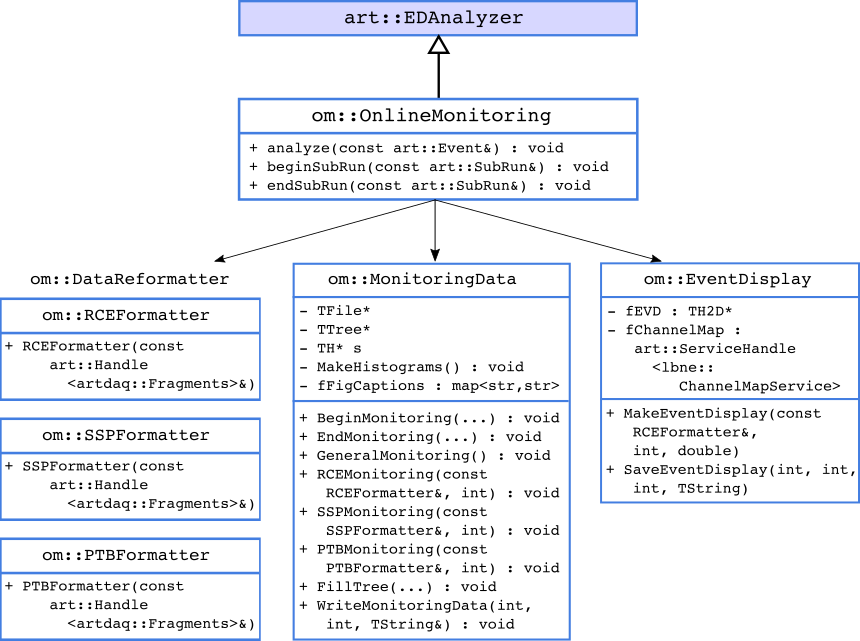
\includegraphics[width=0.8\textwidth]{online_monitoring_software.png}
%\end{cdrfigure}

The DataReformatters restructure the data to allow for efficient subsequent
analysis and provide a standard interface to the methods which look through
the events.  These reformatted objects are passed to MonitoringData, which
owns all of the data products (\texttt{TTree}s, \texttt{TH1}s, \texttt{TGraph}s
etc.) output from the monitoring software and provides methods for filling
them when required.  Finally, the online event displays are
written as part of the monitoring framework, so the EventDisplay class was
responsible for this.  
%This particular functionality will possibly be handled
%differently in ProtoDUNE-SP.
%\fixme{same comment as above - this is not a 35t detector TDR}

The output is then saved in a common area for offline access and for syncing
with a web server. This will be hosted at CERN and will allow for remote
monitoring of the experiment.

\paragraph{Nearline monitoring}

The Nearline Monitoring is designed to provide complimentary information to
that given by the online system. It runs separately as a series of automated
shell scripts and provides feedback on a slower timescale than the online
monitoring, thus allowing for a broader view of the quality of data over time.
It also utilises offline software (LArSoft) to provide, for example,
reconstruction, facilitating a more complete monitoring of much more complex
information.

Once an output data file has been closed by the DAQ, it can be processed by the
nearline system.  A LArSoft job is initially run over the events to perform
reconstruction and extract information from the data.  The output of this,
along with the output of other runs, is then analysed by a separate automated
job, to form the high-level view of the data for monitoring.\\
%
Similar to the online framework, there will be an interface for this system
with the web to allow for remote access of the information.


